\subsection{Backend} % (fold)
\label{sub:backend}

The backend is one of the two parts that make Eagle Eye. Its purpose is to extract information from images and set everything up for the Visualization.

Currently it is a command line utility that allows the user to enter paths for folders containing image files. The system will then read those images, gather their metadata, process them with the existing plugins to extract visual features and, finally, generate and output the multi-scale imagery and the control metadata required by the visualization.

\subsubsection{Architecture of the Backend}

The Backend comprises a library manager to hold the images, feature extractors to process those images and persistence to save all generated data.

The Eagle Eye part is the main application, containing the library and feature extractor managers. Both deal with files on the disk, JPEG image files and DLL extractor plugins, respectively. The user interacts with the core of Eagle Eye which currently provides a command line interface for its actions, like the image import and plugin execution. The import gathers the files and their metadata, to be later accessed by the plugins for processing. Plugins store the resulting data inside the library manager and can be accessed afterwards for outputting by a special plugin.

\begin{figure}[ht]
	\centering
		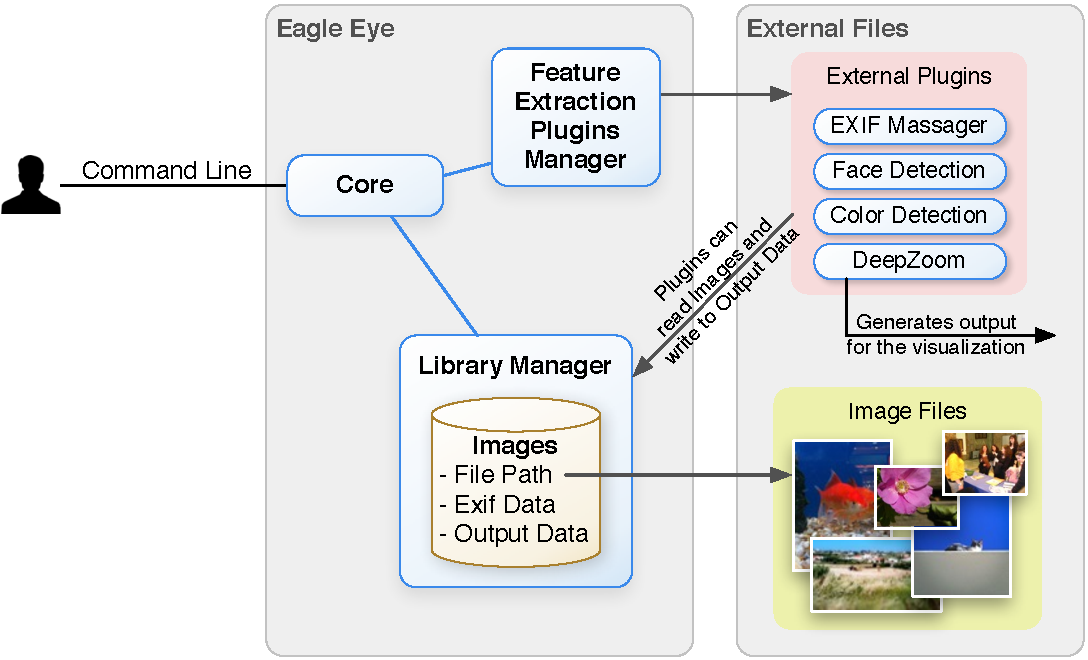
\includegraphics[width=0.8\linewidth]{../Figures/Architecture_v2.pdf}
	\caption{Basic architecture of Eagle Eye's backend}
	\label{fig:arch}
\end{figure}

\subsubsection{Feature Extraction Plugins} % (fold)
\label{sub:plugins}

We will now overview the extractors for the features referred back in Solution Requirements (\ref{reqs:main_goal}).

\textbf{Selection of useful image metadata} This plugin acts as a filter for all the available \ac{EXIF} tags picking the most relevant ones, coding them in a pre-defined way and appending them to the rest of the information to be exported for the visualization.

Timestamp of capture, device, path on disk and keywords are the currently extracted tags.


\textbf{Detection of image’s main color} We looked into a couple of different ways to tackle the color detection extractor but, due to time constraints, we only used a simple method that computes the histogram and returns a median color for each image. It works but induces some errors in images with high contrast.


\textbf{Face Detection} The face detection plugin is based on the open-source OpenCV library\footnote{OpenCV (Open Source Computer Vision) is a library of programming functions for real time computer vision. Available at \url{http://opencv.willowgarage.com}} which processes every image file and detects existing faces.
 
This process is quite computationally expensive and therefore we resize all the images down to a more acceptable size, making the process more than five times faster.


\textbf{Generation of multi-scale imagery}
This plugin generates all the data files needed for the visualization to work. The visualization relies on the DeepZoom technology which needs to process the images before they can be displayed. This plugin does exactly that.

The plugin generates, for each image, a set of image files representing the original one at multiple scales, from a single pixel to a large, detailed image.

After passing through all images, the collection as a whole is processed, this time generating imagery for all images as a single set and a metadata file that agglomerates all image sets used. This metadata file for the collection (called collection.xml) is then altered by the plugin to attach to each image, the data previously generated by the other plugins.

% subsection plugins (end)
